\documentclass{article}
\usepackage[utf8]{inputenc}
\usepackage{amsmath}
\usepackage{amssymb}
\usepackage{amsthm}
\usepackage{amsfonts}
\usepackage{minted}
\usepackage{graphicx}
\usepackage{algorithm}
\usepackage{algorithmic}
\graphicspath{ {img/} }
\usepackage{titlesec}
\usepackage[a4paper,margin=1in,footskip=0.25in]{geometry}
\usepackage{fancyhdr}
\pagestyle{fancy}
%basic page layout

%draw finite state machine
\usepackage{tikz}
\usetikzlibrary{arrows,automata}
\newcommand{\hwnumber}{4}
\newcommand{\Lcvy}{\mathcal{L}}
%header and footer settings
\lhead{Machine Learning \hwnumber}
\chead{Yiping Deng, Shalom-David Anifowoshe}
\rhead{\today}

\titlelabel{\thetitle\enspace}

\begin{document}
\title{Machine Learning \hwnumber}
\author{Yiping Deng, Shalom-David Anifowoshe}
\maketitle
\thispagestyle{fancy}
\section{K-means algorithm}
K-means is a iterative algorithm that basically does the following:
\begin{itemize}
    \item picks $k$ centers(usually done by picking first $k$ data).
    \item groups the dataset by centers
    \item recomputes the centers(taking the mean value)
    \item repeats...
\end{itemize}
Mathematically speaking, for a given sets of clusters,
we have
$ S = \{S_1, S_2, ... S_k\} $ with its corresponding mean 
value $ \bar{X} = \{\bar{x_1}, \bar{x_2}, ... \bar{x_k}\}$. k-means algorithms aims to
$$ \arg\min_{S} \sum_{i = 1}^{k} \sum_{v \in S_i} norm(x, \bar{x_i}) $$
\subsection{$k = 1$}
For $k = 1$, the algorithm calculates the mean value of the vectors. Here the number of iterations were insignificant because it was only making one cluster.  The image below shows the $k  = 1$ case: \\
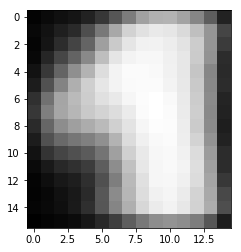
\includegraphics{k_1.png} \\
With $k = 1$, we can prove that the only center will just be the mean value of the set.\\
\begin{proof}
$$ \arg\min_{S} \sum_{i = 1}^{k} \sum_{v \in S_i} norm(x, \bar{x_i}) = \{\{x_1, x_2, ... x_k\}\}$$
Thus, we can conclude the center:
$$ \bar{x_1} = \frac{1}{n} \sum_{i = 1}^{n} x_i $$
Which is exactly the mean value.
\end{proof}
\subsection{$k = 2$}
With this case, the algorithm splits the dataset into two clusters and iteratively computes there centers, here the number of iterations makes a difference because after each iteration the algorithm approaches convergence. \\
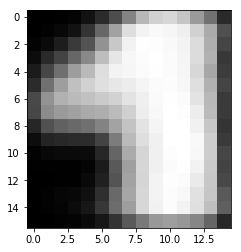
\includegraphics{k_2_1.png} \\
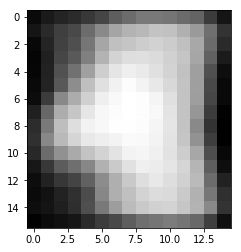
\includegraphics{k_2_2.png} \\
\subsection{$k = 3$}
Very similar logic from the $ k = 2 $ case applies here for the K = 3 case, but however 3 clusters are now being used. The number of iterations is positivly correlated with the likely hood of convergence. \\
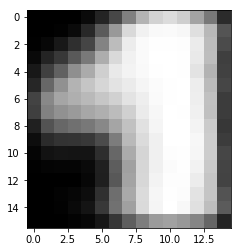
\includegraphics{k_3_1.png} \\
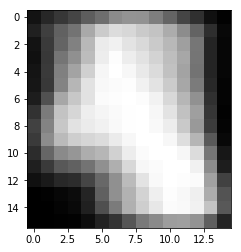
\includegraphics{k_3_2.png}\\
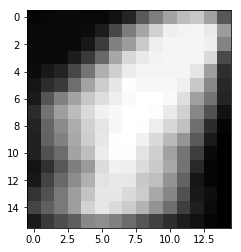
\includegraphics{k_3_3.png}\\
\subsection{$k = 200$}
For the K = 200 case, all 200 points from the data set form their own cluster. Here the distance of each point to it's center is 0 as each cluster is unique to each point. Additionally, here the number of  iterations do not change the output because the algorithm converges after the first iteration.\\
We will simply include 3 graphs here for presentation. \\
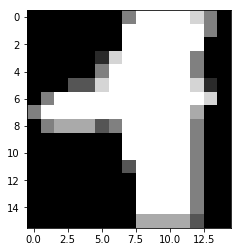
\includegraphics{k_200_1.png} \\
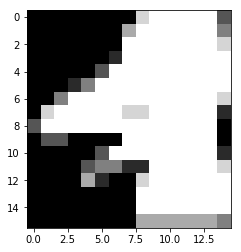
\includegraphics{k_200_2.png} \\
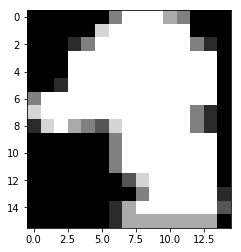
\includegraphics{k_200_3.png} \\
for $k = 200$, clearly $\arg\min$ obtains its minimum 0 at its first iteration.
\begin{proof}
    $$ \arg\min_{S} \sum_{i = 1}^{k} \sum_{v \in S_i} norm(x, \bar{x_i}) = \{\{x_1\}, \{x_2\},... \{x_n\}\} $$
    Thus,
    $$ \bar{x_i} = \frac{1}{1} \sum_{ x \in S_i} x = x_i $$
    Which is picked at its first place.
\end{proof}
\end{document}
